% Options for packages loaded elsewhere
\PassOptionsToPackage{unicode}{hyperref}
\PassOptionsToPackage{hyphens}{url}
%
\documentclass[
]{article}
\usepackage{listings}
\usepackage{amsmath,amssymb}
\usepackage{lmodern}
\usepackage{iftex}
\ifPDFTeX
  \usepackage[T1]{fontenc}
  \usepackage[utf8]{inputenc}
  \usepackage{textcomp} % provide euro and other symbols
\else % if luatex or xetex
  \usepackage{unicode-math}
  \defaultfontfeatures{Scale=MatchLowercase}
  \defaultfontfeatures[\rmfamily]{Ligatures=TeX,Scale=1}
\fi
% Use upquote if available, for straight quotes in verbatim environments
\IfFileExists{upquote.sty}{\usepackage{upquote}}{}
\IfFileExists{microtype.sty}{% use microtype if available
  \usepackage[]{microtype}
  \UseMicrotypeSet[protrusion]{basicmath} % disable protrusion for tt fonts
}{}
\makeatletter
\@ifundefined{KOMAClassName}{% if non-KOMA class
  \IfFileExists{parskip.sty}{%
    \usepackage{parskip}
  }{% else
    \setlength{\parindent}{0pt}
    \setlength{\parskip}{6pt plus 2pt minus 1pt}}
}{% if KOMA class
  \KOMAoptions{parskip=half}}
\makeatother
\usepackage{xcolor}
\IfFileExists{xurl.sty}{\usepackage{xurl}}{} % add URL line breaks if available
\IfFileExists{bookmark.sty}{\usepackage{bookmark}}{\usepackage{hyperref}}
\hypersetup{
  hidelinks,
  pdfcreator={LaTeX via pandoc}}
\urlstyle{same} % disable monospaced font for URLs
\usepackage{graphicx}
\makeatletter
\def\maxwidth{\ifdim\Gin@nat@width>\linewidth\linewidth\else\Gin@nat@width\fi}
\def\maxheight{\ifdim\Gin@nat@height>\textheight\textheight\else\Gin@nat@height\fi}
\makeatother
% Scale images if necessary, so that they will not overflow the page
% margins by default, and it is still possible to overwrite the defaults
% using explicit options in \includegraphics[width, height, ...]{}
\setkeys{Gin}{width=\maxwidth,height=\maxheight,keepaspectratio}
% Set default figure placement to htbp
\makeatletter
\def\fps@figure{htbp}
\makeatother
\usepackage[normalem]{ulem}
% Avoid problems with \sout in headers with hyperref
\pdfstringdefDisableCommands{\renewcommand{\sout}{}}
\setlength{\emergencystretch}{3em} % prevent overfull lines
\providecommand{\tightlist}{%
  \setlength{\itemsep}{0pt}\setlength{\parskip}{0pt}}
\setcounter{secnumdepth}{-\maxdimen} % remove section numbering
\ifLuaTeX
  \usepackage{selnolig}  % disable illegal ligatures
\fi

\author{}
\date{}

\begin{document}

\hypertarget{why-cyclegan}{%
\section{Why "CycleGAN"?}\label{why-cyclegan}}

The reason it is called a cycleGAN is that we will use the two GAN
models to construct a cycle for some purpose. To make such cycle, we
need to make the two GAN models to do exactly the same work, that is to
do \emph{image-to-image translation}, but in reversed directions.
Specifically, we want GAN A to transfer a horse image to a zebra image,
while GAN B has the ability to transfer a zebra image to a horse image.
Each of the two GAN models is formed by a Conditional Generator and a
PatchGAN Discriminator. We will talk about the structures of the
generator and discriminators in the following section. To sum up, in our
tool box we have two GAN models. Each of them contains one generator and
one discriminator.

\hypertarget{why-two-gans}{%
\subsection{Why two GANs?}\label{why-two-gans}}

The major advantage of a cycleGAN: it won't require
\protect\hyperlink{one-merit-of-paired-samples}{pair samples} anymore in
the training process.

\hypertarget{one-merit-of-paired-samples}{%
\subsection{One merit of paired
samples}\label{one-merit-of-paired-samples}}

They put strict restriction on the generated images so that except the
desired adjustments (e.g. zebra pattern), the rest part of the generated
images will be unchanged from the source images.

Although we take this restriction for granted when we have paired
samples because it comes naturally with the strongly correlated paired
images, it is not the case anymore when we switch to unpaired samples
where there is no correlation between source images and target images.

\hypertarget{cycle-consistency}{%
\section{\texorpdfstring{Cycle Consistency
}{Cycle Consistency }}\label{cycle-consistency}}

Put the restriction back on generated images through an additional loss
function.

\begin{quote}
We exploit the property that translation should be ``cycle consistent'',
in the sense that if we translate, e.g., a sentence from English to
French, and then translate it back from French to English, we should
arrive back at the original sentence.

--- Unpaired Image-to-Image Translation using Cycle-Consistent
Adversarial Networks, 2017.
\end{quote}

\uline{All we need to do then is convert the difference between the two
horse images to a loss function.}

This process is called Forward Cycle, a half of the cycle structure
which focuses on evaluating GAN A. The other half of the cycle, which is
called Backward Cycle, will have exactly the same workflow of its
counterpart but in a reversed direction so that it could evaluates GAN
B.

Combining the two loss functions from Forward and Backward Cycles, we
obtain a general \textbf{loss function} called \emph{Cycle Consistency}
Loss and we will involve it as a part of the final loss function which
we will use to update the cycleGAN model.

\hypertarget{identity-loss}{%
\section{Identity Loss}\label{identity-loss}}

While the outcome zebras seem to have the same shape and other stuff
with the input horses under cycle consistency restriction, the color
profile consistency between inputs and outputs was not maintained very
well by the model.

To solve this problem, they invented another structure called
\textbf{Identity Mapping}.

\begin{quote}
One of them focuses on the performance of GAN A and the other one
evaluates GAN B.

To evaluate GAN A, for example, instead of feeding it with a horse
image, we will give it a zebra image.

By its nature, GAN A will generate a new zebra image based on the
original zebra. Ideally, all the stuff laying on the two images,
including the colors, \uline{should look exactly the same}.
\end{quote}

\hypertarget{loss-function}{%
\subsection{Loss function}\label{loss-function}}

Again, we convert the difference between the two images to a loss
function and combine it with the loss function from the other components
to form an Identity Loss function, which will also be a part of the
final loss function.

\hypertarget{discriminator}{%
\section{Discriminator}\label{discriminator}}

A fully CNN with totally five layer blocks where each block contains a
2D Convolution Layer with kernel size of 4x4 and stride of 2, an
Instance Normalization Layer and a Leaky ReLU Layer (except the output
block which uses a Sigmoid Layer as activation).

\begin{figure}
\centering
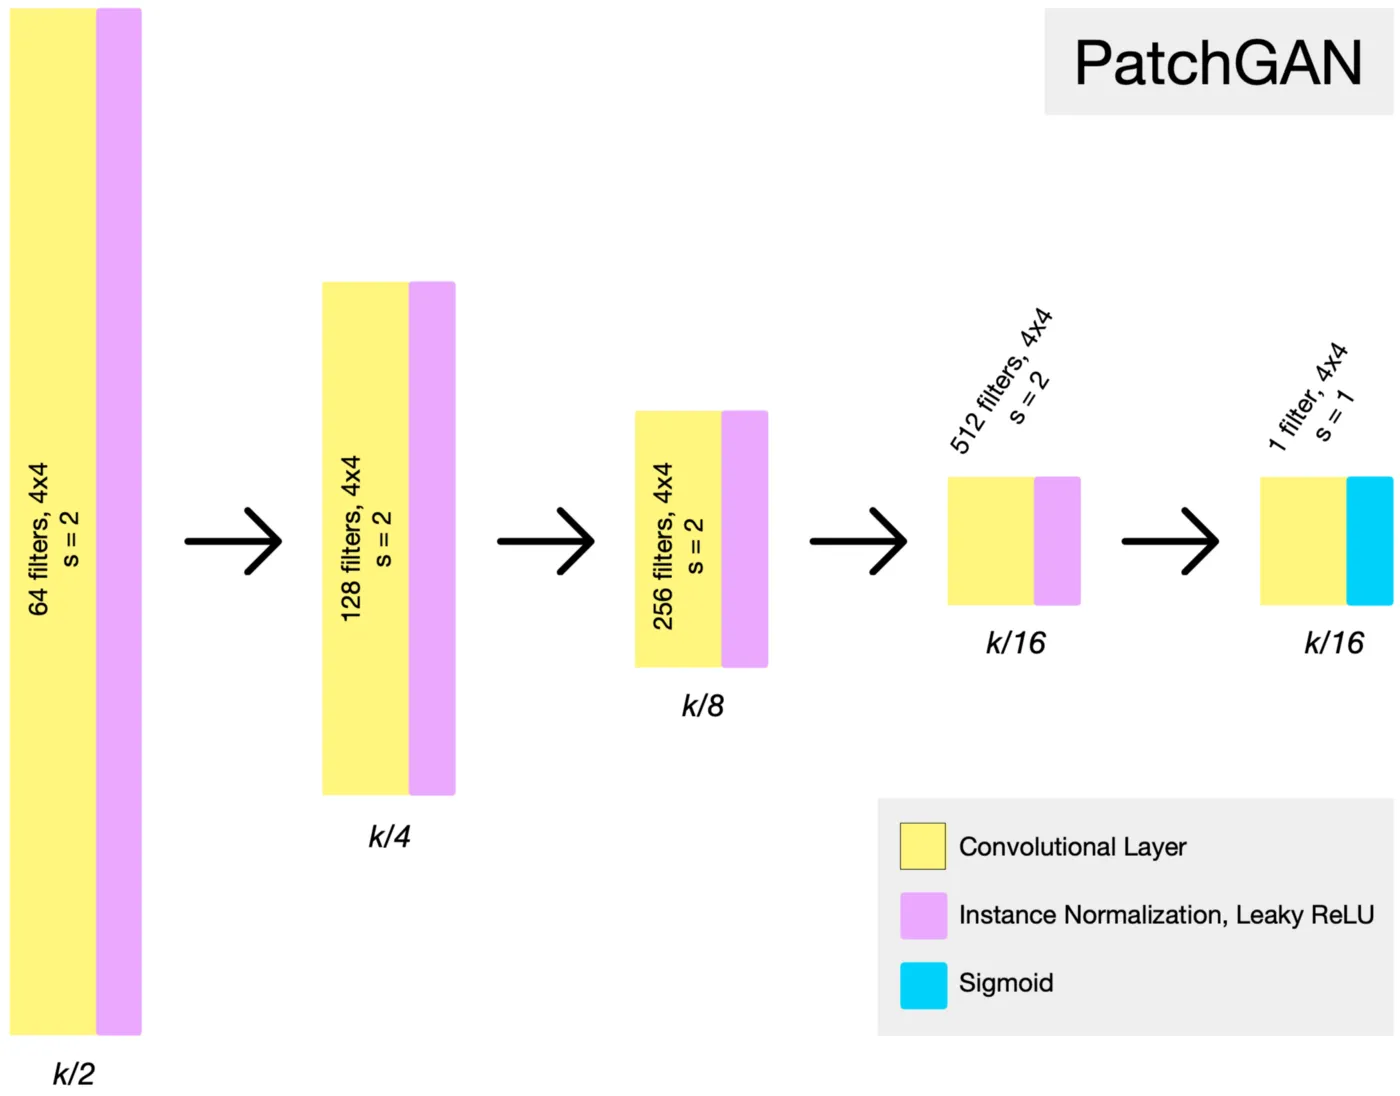
\includegraphics{./assets/PatchGAN.png}
\caption{PatchGAN}
\end{figure}

\hypertarget{why-16-uxd7-16-matrix-}{%
\subsection{Why 16 × 16 matrix ?}\label{why-16-uxd7-16-matrix-}}

This is because in cycleGAN, we are using a structure called PatchGAN
for the discriminator.

Unlike a normal discriminator which takes \uline{an image as a whole} to
judge whether it is real or fake, \uline{a PatchGAN discriminator will
first divide the input image into a number of ``patches'' and then make
\emph{\textbf{individual judgements}} on each of them}.

In our case, the input image is divided into 16x16 patches in the end
where each patch has a size of 70x70.

\hypertarget{generator}{%
\section{Generator}\label{generator}}

A neural network structure which is formed by three sections:

\begin{itemize}
\item
  Encoder

  \begin{itemize}
  \item
    Layer block × 3

    \begin{quote}
    The first layer block doesn't change the size of image, it only
    creates 64 channels on the input. The next two layer blocks however,
    each shrinkages the input size by half while also double the number
    of channels.
    \end{quote}

    \begin{itemize}
    \item
      2D Convolution Layer × 1
    \item
      Instance Normalization Layer × 1
    \item
      Leaky ReLU Layer × 1
    \end{itemize}
  \end{itemize}
\item
  Transformer

  \begin{itemize}
  \item
    ResNet × 6

    each contains
    
    \begin{itemize}
    \item
      Layer block × 2

      \begin{itemize}
      \item
        2D Convolution Layer (with stride=1) × 1
      \item
        Instance Normalization Layer × 1
      \item
        Leaky ReLU Layer. × 1
      \end{itemize}

      and

      \begin{itemize}
      \item
        2D Convolution Layer (with stride=1) × 1
      \item
        Instance Normalization Layer × 1
      \end{itemize}
    \end{itemize}
  \end{itemize}
\item
  Decoder

  \begin{quote}
  The decoder enlarges the input back to the original size and collapses
  all channels into RGB to form the final output image.
  \end{quote}

  \begin{itemize}
  \item
    \href{https://machinelearningmastery.com/upsampling-and-transpose-convolution-layers-for-generative-adversarial-networks/}{Transpose
    Convolution Layers} × 2

    \begin{quote}
    Enlarge the size of input while decrease the number of channels
    \end{quote}
  \item
    Output layer × 1

    \begin{quote}
    Collapse the channels into RGB and thus output it as the final
    output image
    \end{quote}
  \end{itemize}
\end{itemize}

\begin{figure}
\centering
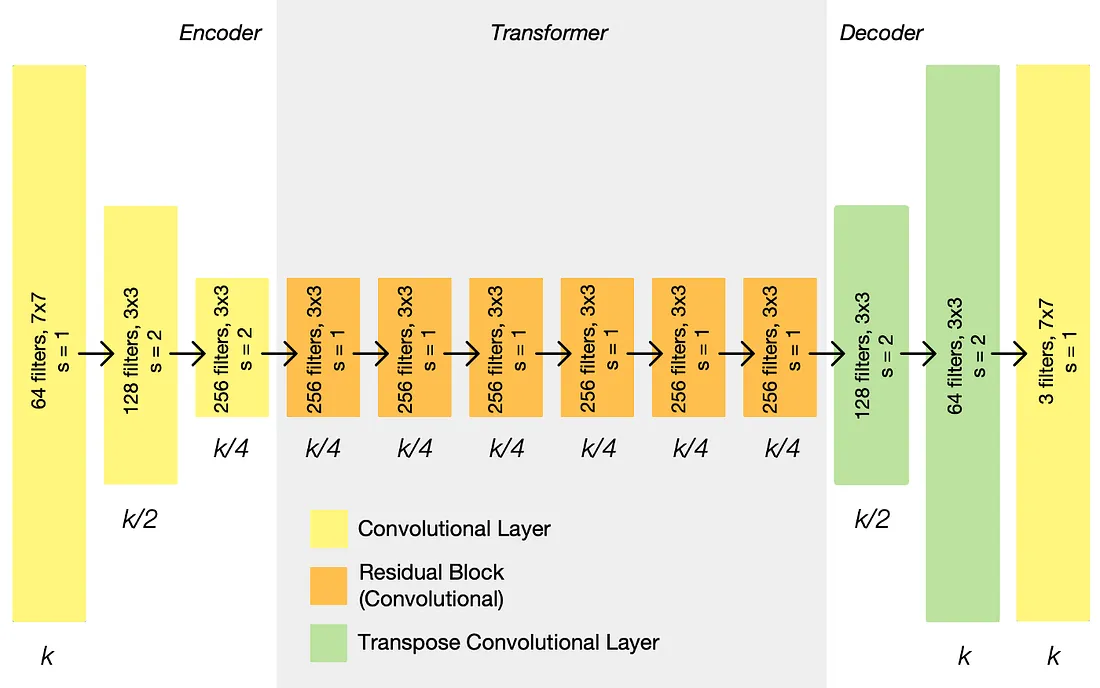
\includegraphics{./assets/Generator.png}
\caption{Generator}
\end{figure}

\hypertarget{update-weight-for-a-generator-through-a-composite-model}{%
\section{Update Weight for a Generator Through a Composite
Model}\label{update-weight-for-a-generator-through-a-composite-model}}

\begin{quote}
Traditionally, a composite model generates only one loss function ---
the \uline{\emph{\textbf{adversarial loss}}} which reflects how well the
discriminator identifies fake images produced by the generator.
\end{quote}

For a cycleGAN generator, however, there are three other loss functions
should be involved --- the \uline{\emph{\textbf{identity loss}}} and
\uline{\emph{\textbf{forward/backward consistency loss}}}.

There are 4 independent components which produces the 4 loss functions.

While the \uline{\emph{\textbf{adversarial loss}}} is represented by L2
loss function (Mean Square Error, MSE), the rest three are represented
by L1.

The four losses are weight averaged to obtain the final loss function:
\uline{The \emph{\textbf{cycle consistency loss}} has the highest weight
while the effect from \emph{\textbf{adversarial loss}} is downplayed.}

At the end of each iteration, we record the final loss function and use
Adam SGD to update model weight of the generator.

\begin{figure}
\centering
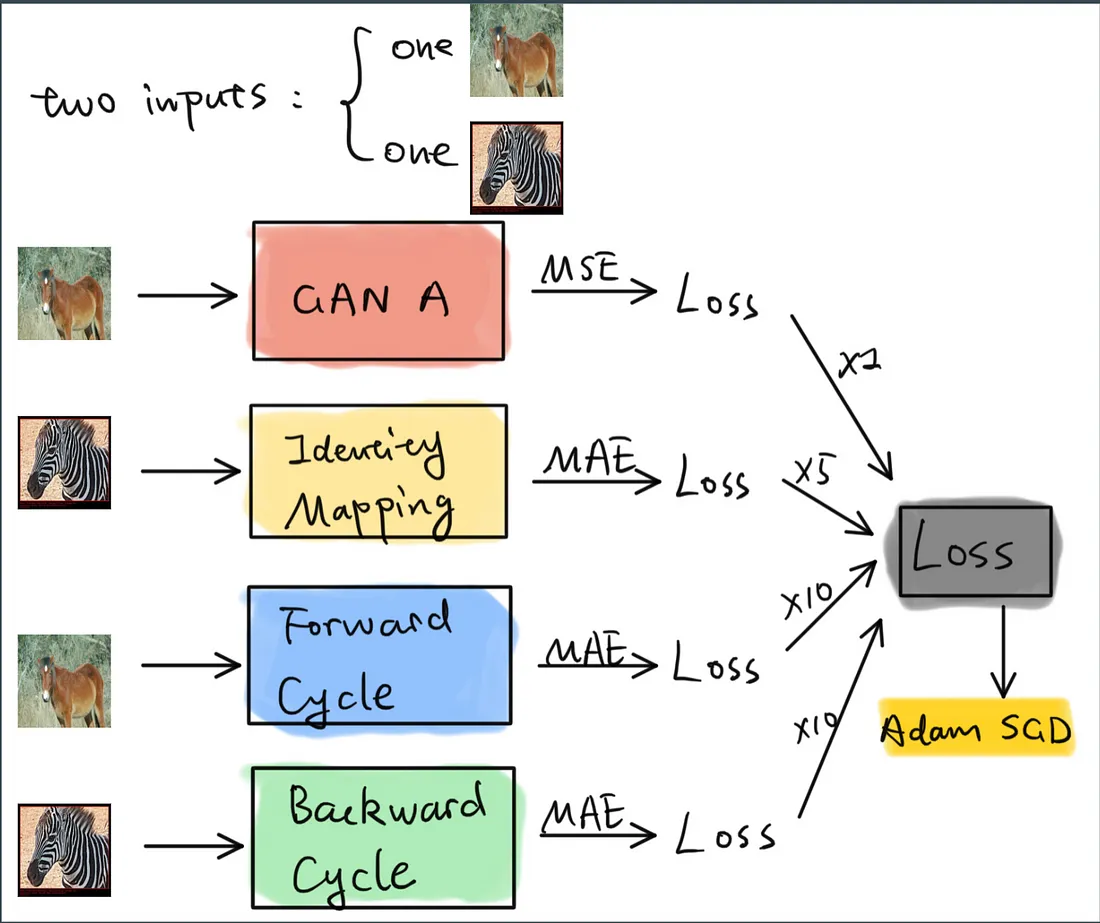
\includegraphics{./assets/Update_Weights.png}
\caption{Update Weights}
\end{figure}

\hypertarget{adversarial-loss}{%
\subsection{Adversarial Loss}\label{adversarial-loss}}

For the mapping function \(G:X \rightarrow Y\) and its discriminator \(D_Y\),
we express the objective as:

\[\mathcal{L}_{\text{GAN}}(G,D_Y,X,Y)=\mathbb{E}_{y\sim p_{\text{data}}(y)}[\log{D_y(y)}]+\mathbb{E}_{x\sim p_{\text{data}}(x)}[\log{(1-D_y(G(x)))}]\]

where \(G\) tries to generate images \(G(x)\) that look similar to
images from domain \(Y\), while \(D_Y\) aims to distinguish between
translated samples \(G(X)\) and real samples \(y\).

\hypertarget{cycle-consistency-loss}{%
\subsection{Cycle Consistency Loss}\label{cycle-consistency-loss}}

\begin{figure}
\centering
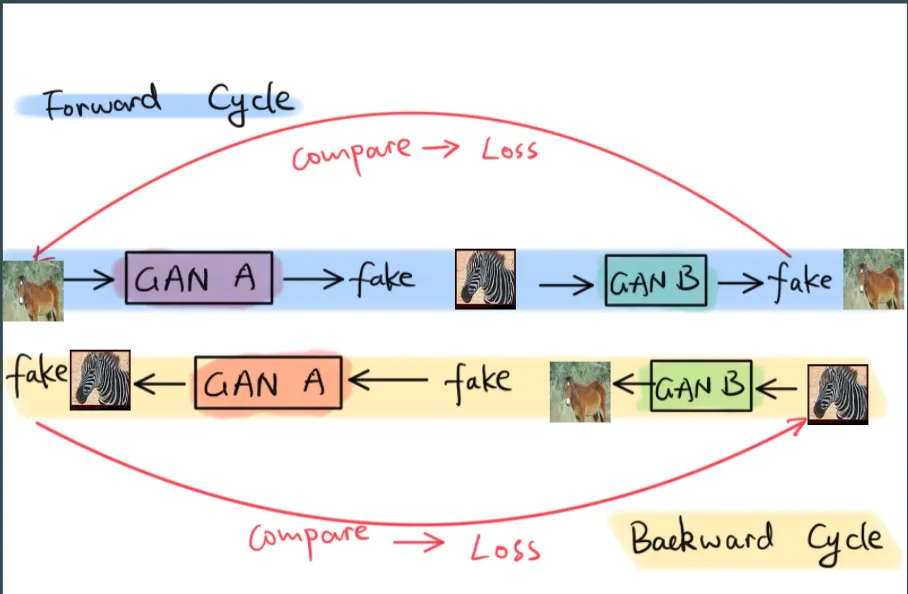
\includegraphics{./assets/cycle_consistency_loss.png}
\caption{Cycle Consistency Loss}
\end{figure}

\hypertarget{forward-cycle-consistency}{%
\subsubsection{Forward cycle
consistency}\label{forward-cycle-consistency}}

\[\mathcal{L}_{\text{cyc}}(G,F)=\mathbb{E}_{x\sim p_{\text{data}}(x)}[\left\|F(G(x))-x\right\|_1]+\mathbb{E}_{y\sim p_{\text{data}}(y)}[\left\|G(F(y))-y\right\|_1]\]

Functions should be cycle-consistent: for each image \(x\) from domain
\(X\), the image translation cycle should be able to bring \(x\) back to
the original image.

\[x\rightarrow G(x)\rightarrow F(G(x))\approx x\]

\hypertarget{backward-cycle-consistency}{%
\subsubsection{Backward cycle
consistency}\label{backward-cycle-consistency}}

Similarly, for each image \(y\) from domain \(Y\), \(G\) and \(F\)
should also satisfy backward cycle consistency:

\[y\rightarrow F(y)\rightarrow G(F(y))\approx y\]

\hypertarget{identity-loss-2}{%
\subsection{Identity Loss}\label{identity-loss-2}}

\begin{quote}
It is an additional loss to encourage the mapping to preserve color
composition between the input and output.
\end{quote}

\[\mathcal{L}_{\text{identity}}(G,F)=\mathbb{E}_{y\sim p_{\text{data}}(y)}[\left\|G(y)-y\right\|_1]+\mathbb{E}_{x\sim p_{\text{data}}(x)}[\left\|F(x)-x\right\|_1]\]

\hypertarget{full-object}{%
\subsection{Full object}\label{full-object}}

\[\mathcal{L}(G,F,D_X,D_Y)=\mathcal{L}_{\text{GAN}}(G,D_Y,X,Y)+\mathcal{L}_{\text{GAN}}(F,D_X,Y,X)+\lambda \mathcal{L}_{\text{cyc}}(G,F)\]

\hypertarget{update-weight-for-a-discriminator-using-image-pool}{%
\section{Update Weight for a Discriminator Using Image
Pool}\label{update-weight-for-a-discriminator-using-image-pool}}

An \textbf{image pool} is a set of at most 50 fake images produced by
the generator in the past iterations.

The goal of image pools is to
\href{https://towardsdatascience.com/cyclegan-learning-to-translate-images-without-paired-training-data-5b4e93862c8d}{prevent
cycleGAN model from changing drastically from iteration to iteration}.

\begin{figure}
\centering
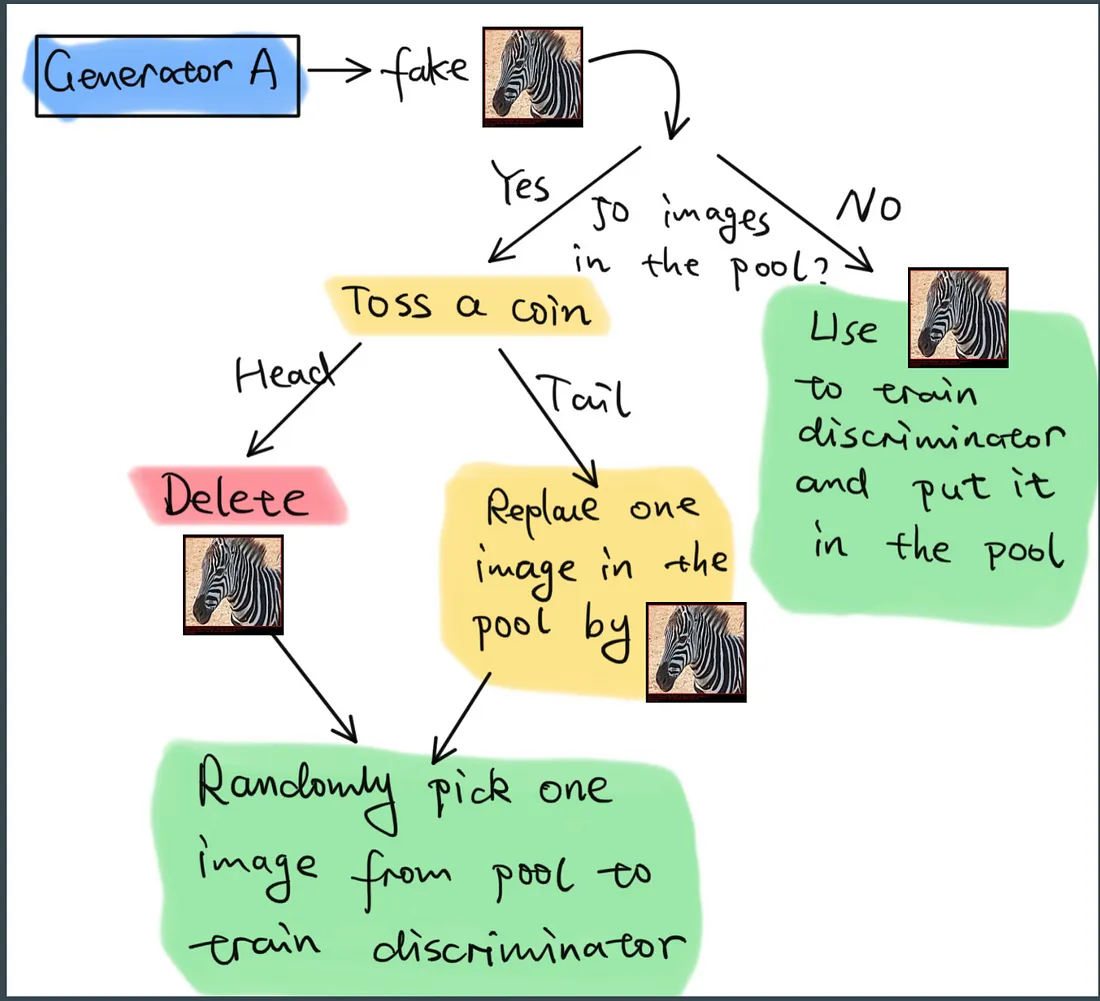
\includegraphics{./assets/Update_Weight_for_a_Discriminator.png}
\caption{Update Weight for a Discriminator}
\end{figure}

Once we have the two images ready, all we need to do is put them to the
discriminator separately and sum up the two loss functions represented
by L2. We record the loss sum and update the weight of the discriminator
using Adam SGD.

\newpage

Todo and summary:

\begin{figure}
\centering
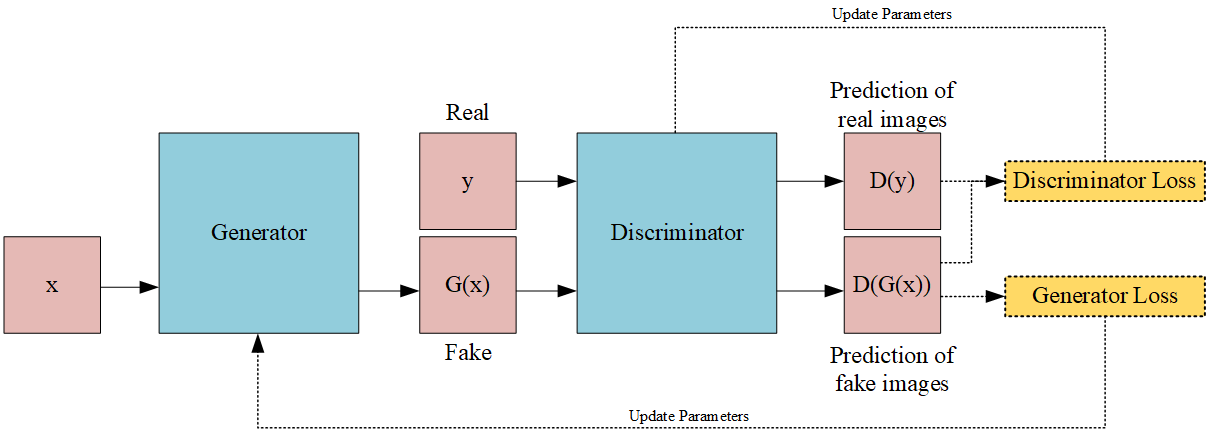
\includegraphics{./assets/GAN.png}
\caption{}
\end{figure}

\begin{enumerate}
\def\labelenumi{\arabic{enumi}.}
\item
  Which is the subject of the Adversarial Loss function expression
  L\_GAN? Which is the accompaniment?

  \[\mathcal{L}_{\text{GAN}}(G,D_Y,X,Y)=\mathbb{E}_{y\sim p_{\text{data}}(y)}[\log{D_y(y)}]+\mathbb{E}_{x\sim p_{\text{data}}(x)}[\log{(1-D_y(G(x)))}]\]

  In the above equation, we notice that during the training of the
  \textbf{discriminator (D)} focuses on maximizing the \(\log{D_y(y)}\),
  which means achieving the correct label during the classification of
  \(y\) and maximizing the \(\log{(1-D_y(G(x)))}\), which means trying
  to identify the fake image. The \textbf{generator (G)} focuses on
  minimizing \(\log{(1-D_y(G(x)))}\), and cannot directly influence
  \(\log{D_y(y)}\). So the term
  \(\mathbb{E}_{x\sim p_{\text{data}}(x)}[\log{(1-D_y(G(x)))}]\) is the
  subject.

  \begin{quote}
  The above minimax loss function can cause the GAN to get stuck in the
  early stages of GAN training when the discriminator's job is very
  easy. It is suggested to modify the generator loss so that the
  generator tries to maximize \(\log D(G(z))\).
  \end{quote}
\item
  Decompose the process of L\_GAN. What is the relationship between
  L\_cyc and L\_GAN ?

  \begin{itemize}
  \item
    The generator's objective is to fool the discriminator, another
    component of the GAN, into classifying its generated samples as
    real. The generator loss measures the dissimilarity between the
    predicted probability by the discriminator for the generated data
    and the desired label of "real" (1).

    \[\text{Generator Loss: } \mathcal{L}_G = \frac{1}{n}\cdot\sum_i^n \log{(1-D(G(x)))}\]
  \item
    While the discriminator is trained, it classifies both the real data
    and the fake data from the generator.

    \[\text{Discriminator Loss: } \mathcal{L}_D= -\log(D(y)) - \log(1 - D(G(x)))\]

    \begin{itemize}
    \item
      The first cross-entropy term, \(-\log(D(y))\), measures the
      difference between the discriminator's probability of classifying
      real samples \(y\) as real and the true labels. \uline{This
      cross-entropy term encourages the discriminator to correctly
      categorize the true sample as true.}
    \item
      The second cross-entropy term \(-\log(1 - D(G(x)))\) is the
      cross-entropy for the generated sample \(G(x)\). It measures the
      difference between the probability that the discriminator
      classifies the generated sample \(G(x)\) as a true sample and the
      generated sample label (i.e., not present). This cross-entropy
      term encourages the discriminator to correctly categorize
      generated samples as generated samples (i.e., false samples).
    \end{itemize}
  \end{itemize}

The basic idea of Cycle Consistency is to learn simultaneously the mapping from distribution X to Y and from Y to X in a generative model, given two different data distributions X and Y. This is achieved by enforcing a bi-directional consistency constraint. It means that for any sample x from X, mapping it to Y space and then back to X space should preserve the similarity to the original sample x. Similarly, for any sample y from Y, mapping it to X space and then back to Y space should preserve the similarity to the original sample y.

Through this adversarial training, the generator can learn to generate high-quality synthetic samples.

\[\mathcal{L}_{\text{cyc}}(G,F)=\mathbb{E}_{x\sim p_{\text{data}}(x)}[\left\|F(G(x))-x\right\|_1]+\mathbb{E}_{y\sim p_{\text{data}}(y)}[\left\|G(F(x))-y\right\|_1]\]

\item
  Now that L\_GAN and L\_cyc are available, there are still some
  problems with the performance of the network. Forget the Identity loss
  in the article, how do I modify this current loss function?
\item
  Figure out the Identity loss.
  
\[\mathcal{L}_{\text{identity}}(G,F)=\mathbb{E}_{y\sim p_{\text{data}}(y)}[\left\|G(y)-y\right\|_1]+\mathbb{E}_{x\sim p_{\text{data}}(x)}[\left\|F(x)-x\right\|_1]\]

Identity loss is a loss function used in training generative models. It is commonly employed in tasks such as face recognition, pose estimation, etc., with the aim of ensuring that the generated outputs have the same identity information as the inputs.

In Identity loss, the objective of the generator is to produce outputs that are similar to the inputs, thereby maintaining consistency in identity information. To achieve this, a distance metric is often used to measure the difference between the generated results and the inputs, such as Euclidean distance or cosine similarity. The loss function of Identity loss minimizes this difference, striving to make the generated results as consistent as possible with the inputs.

\item
  Feed some special images to the model and debug the value of each loss
  function. Try to find abnormal values.
\end{enumerate}

\hypertarget{code-analysis}{%
\section{Code analysis}\label{code-analysis}}

\begin{lstlisting}[language=Python]
self.criterionGAN = networks.GANLoss(opt.gan_mode).to(self.device)
self.criterionCycle = torch.nn.L1Loss()
self.criterionIdt = torch.nn.L1Loss()
\end{lstlisting}

\begin{itemize}
  \item self.criterionGAN is a GAN loss function, used to train the generator and discriminator during training.
  
  \item self.criterionCycle is a L1 loss function:\[\mathcal{L}_{\text{cyc}}(G,F)=\mathbb{E}_{x\sim p_{\text{data}}(x)}[\left\|F(G(x))-x\right\|_1]+\mathbb{E}_{y\sim p_{\text{data}}(y)}[\left\|G(F(y))-y\right\|_1]\]
  
  \item self.criterionIdt is the Identity loss:\[\mathcal{L}_{\text{identity}}(G,F)=\mathbb{E}_{y\sim p_{\text{data}}(y)}[\left\|G(y)-y\right\|_1]+\mathbb{E}_{x\sim p_{\text{data}}(x)}[\left\|F(x)-x\right\|_1]\]
  
\end{itemize}

Loss during training process(To be continued):
\begin{figure}
\centering
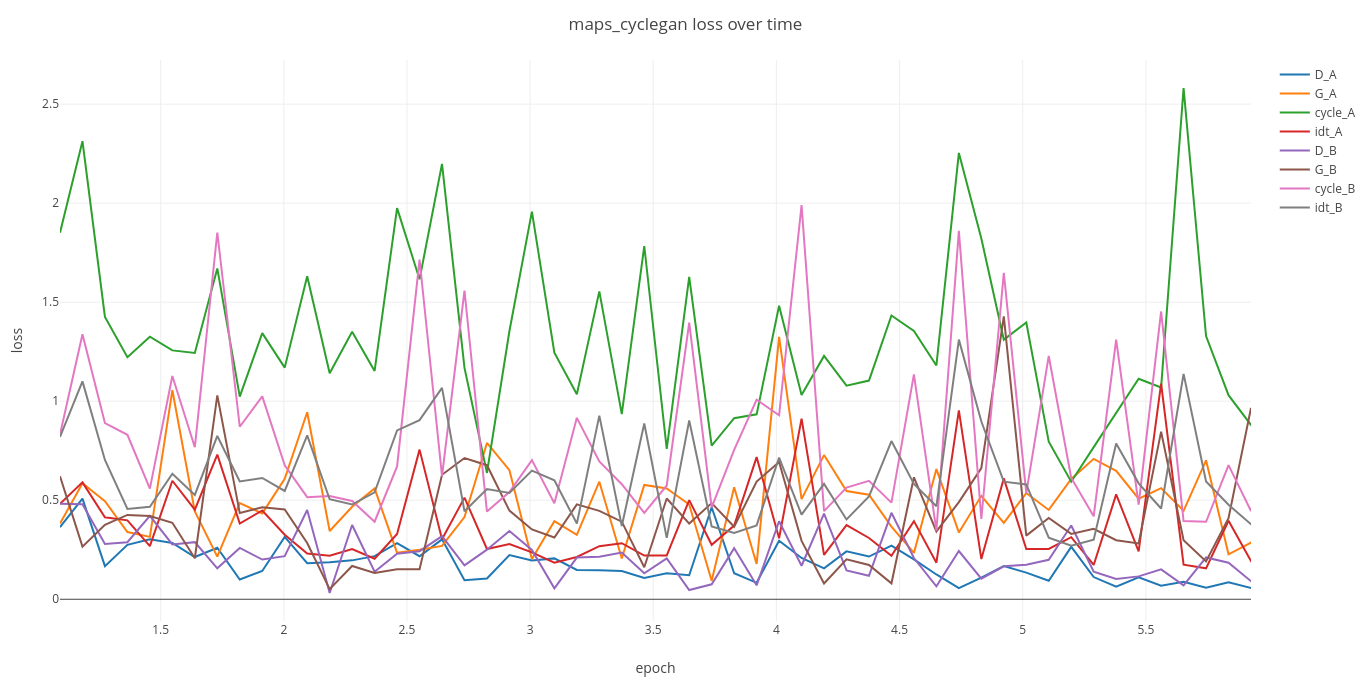
\includegraphics{./assets/Loss_over_time.png}
\caption{Loss over time}
\end{figure}

\end{document}
